\documentclass[12pt]{beamer}
\usetheme{Goettingen}

% Possible Stuff
%   - Karatsuba's Geschichte mit dem Prof

% Begin Outline
% + Be fruitful and multiply
% + Motivation
%   + Wo wird Karatsuba genutzt:
%     + CPython Corelib
%     + Ueberall, wo GMP genutzt wird, wird quasi Karatsuba genommen
%     + Haskell Integer-Implementation
% - Prerequisites
%   + Definition Multiprecision integer
%     - 64bit CISC modern, somit ist das der absolut höchste basecase, bei schlauen SIMD sogar noch höher
%     - Alle Anmerkungen im ORG-MODE
%   + Definition Ring
%   + Definition Kommutativer Ring mit 1
%   + Definition Discrete Convolution
%     + Überleitung dass wir es jetzt direkt nutzen
%   + Definition Polynomring
%     + Erklären warum wir bei Polynomen bleiben
%       + More generic
%       + Easier time complexity analysis
%       + Also, it makes it easier to show the length of something
% ~0:00
% + Naive Algorithm
%   + Ein Beispiel
%   + Saloppe Komplexitätsanalyse
% - Karatsuba
%   + Example without Recursion ab*cd
%   + This takes 2* 1/2 O(n^2). We can use recursion!
%   + Algorithm
%     + T(n) = 4T(n/4) + Theta(n)
% ~1:00
% + Analysis
%   + Herleitung Mastertheorem
%     + Sehr viel Publikumsinteraktion
%     + Noch nicht erklären dass es tatsächlich das Mastertheorem ist
%   + Erklärung, dass es das Mastertheorem ist
%   - Beweis Mastertheorem Fall 1
%     - Fuer Restliche Faelle siehe Manea Info3 oder CLRS
%   + ...
%   + Zusammenfassung Mastertheorem
% + Laufzeitanalyse, the easy way
%   + Anwendung Mastertheorem Karatsuba
% ~3:00
% - A generalized Toom-Cook approach
%   - Overviewfolie, dass es nur eine Generalisierung ist, wir nutzen nur toom 3
%   - Sketch out how it works, 5 steps
%     - Hier erklaeren wann Sachen O(1) sind da die Multiplikationsgroesse nicht davon abhaengig ist
%   - Laufzeitanalyse Toom Cook
% - Beyond Karatsuba Offman
%   - Recap: Polynomringe und Multiplikationen sind Convolutions
%   - Definition FFT
%   - Convolution Theorem
%   - Laufzeitenverbesserungen
%   - Why is Karatsuba still being used then?
%     - Wie wir an Karatsuba/Toom gesehen haben wird je niedriger die Komplexitaet desto hoeher die Konstante
%     - Zitat vom letzten Paper ab welcher Menge an Digits es sich lohnt umzusteigen.
%   - Was es noch fuer Erkenntnisse gab
% - What did we learn?
%   - When numbers are big, at least use Karatsuba
%     - In reality, just use the GMP-Implementation
%   - When you are born early enough, you get a theorem named after you
%   - The Master Method is your best friend when dealing with complexity :)
% - Quellen
% - Ende
% ~4:00
% - Working off TODOs
% ~4:30

% Math Packages
\usepackage{amsmath,amsthm,amssymb,amsfonts}
% More advanced <ol>'s
\usepackage{enumerate}
% Simple Code formatting, no syntax highlighting
\usepackage{listings}
% \mathclap
% See: https://pbelmans.ncag.info/blog/2010/12/06/the-power-of-mathclap-and-substack/
\usepackage{mathtools}
% Graphic Packages
% Also, we use the "float" package for \begin{figure}[H].
% The H-Parameter is described as follows:
%
% Places the float at precisely the location in the LaTeX code. Requires the `float` package, though it may cause
% problems occasionally. This is somewhat equivalent to `h!`.
%
% See: https://de.overleaf.com/learn/latex/Inserting_Images
\usepackage{graphicx}
\usepackage{float}
% \say{}
\usepackage{dirtytalk}
% Hyperlinks
\hypersetup{colorlinks = true, linkcolor = blue, urlcolor = blue, citecolor = blue, anchorcolor = blue}

% TODO: Think of a cooler title
% TODO: Change the colour scheme
% TODO: Move \usepackage's to Dotfiles with description
% TODO: Check for spelling and whether dots are everywhere
% TODO: Think where to add pauses
% TODO: Review Lecture notes
% TODO: Check all Frameheadlines
% TODO: Check whether the def/theorem enumerations are correct
% TODO: Note that polys make it easier; How polys with base 10 are numbers; with base 2^{64} are word-based
% TODO: Break up the schriftliche multiplications into multiple tables
% TODO: Scan the whole document for TODOs CTRL-F-ish
% TODO: proof read everything
% TODO: If we have some time left, do the master theorem proof for case 1

% Quellen:
% - Alle Hyperlinks
% - Wikipedia Ring/Commutative Ring/Convolutions


\title{Fast Long Integer Multiplication in an Pre-FFT Era}
\author{Lars Quentin}
\institute{University of G\"ottingen}
\date{November 18, 2021}

\begin{document}

\frame{\titlepage}

\begin{frame}{}
\begin{center}
{\Huge \say{Be fruitful and multiply}}\\
Genesis 1:28
\end{center}
\end{frame}

\begin{frame}{Overview}
\tableofcontents
\end{frame}

\section{Motivation}



% Talking Points:
% - Explizit erwaehnen dass es sich hierbei um Hyperlinks zu Source Code oder Docs handelt
% - GMP = GNU Multiple Precision Arithmetic Library
\begin{frame}{}
\begin{block}{Where is Karatsuba's Algorithm used nowadays?}
\begin{itemize}
\item \href{https://docs.python.org/3/library/decimal.html}{CPython} uses Karatsuba's multiplication
\begin{itemize}
\item Also \href{https://docs.python.org/3/library/decimal.html}{PyPy3}
\end{itemize}
~\\
\item The \href{https://github.com/ghc/ghc/blob/master/libraries/integer-gmp/src/GHC/Integer/GMP/Internals.hs}{Glassgow Haskell Compiler} uses Karatsuba/Toom-3 for Multiplication.\\~\\
\item The \href{https://en.wikipedia.org/wiki/GNU\_Multiple\_Precision\_Arithmetic\_Library}{GMP} Library is used in all of HPC.
\begin{itemize}
\item It automatically uses Karatsuba/Toom Cook for medium sized numbers.
\item See: \href{https://doi.org/10.3390/math3020337}{\say{High-Precision Arithmetic in Mathematical Physics}} for applications.
\end{itemize}
\end{itemize}
\end{block}
\end{frame}

\section{Prerequisites}

% Talking Points:
% - CISC = Complex Instruction Set Computer
% - Note: Integers are represented in radix 2
\begin{frame}{Integer Represenation 1}
\begin{itemize}
\item Processors are computating data in chunks of a certain size, so called \emph{words}.
\begin{itemize}
\item Since the word size is constant, all elementary operations can be (and are) implemented in $O(1)$
\end{itemize}
\item In modern CISC architecture the default word size is $64$ bits
\begin{itemize}
\item i.e for Integers: $\{0,\dots, 2^{64} -1\}$
\end{itemize}
\item Often, this is not enough. Thus we now define \emph{multiprecision integers}:
\end{itemize}
\end{frame}

% Talking Points:
% - One could use one more word with a single used bit for signed numbers with (-1)^s
%   - Draw in slide for that
% - One can think of it like normal numbers but in base 2^{64}
% - After: It will make things easier when we
\begin{frame}{Integer Represenation 2}
\begin{block}{Definition 1: Multiprecision Integer}
The \emph{multiprecision integer} $a \in \mathbb{N}$ is represented as a vector of \emph{words} $a_i$ such that
\[
a = \sum_{0 \leq i \leq n} a_i \cdot 2^{64i}
\]
where $n \in \mathbb{N}$, $a_i \in \{0, \dots, 2^{64} -1 \}$ for all digits $i$.
\end{block}
\end{frame}

% Talking points:
% - Ellaborate on associativity...
\begin{frame}{Some more formality...}
\begin{block}{Definition 2: Ring}
A \emph{ring} $(R, +, \cdot)$ is a set $R$ with 2 binary operations $+$ and $\cdot$ which satify
the following axioms.
\begin{enumerate}
\item $(R, +)$ is an abelian group under addition, meaning that
\begin{itemize}
\item $+$ is associative
\item $+$ is commutative
\item There is a neutral element $0 \in R$
\item Every element has an additive inverse
\end{itemize}
\item $(R, \cdot)$ is a semigroup under multiplication, meaning that $\cdot$ is associative
\item Multiplication is distributiove with respect to addition, i.e. $\forall a,b,c \in R$
\[
a \cdot (b+c) = (a\cdot b) + (a \cdot c)
\]
\end{enumerate}
\end{block}
\end{frame}

% Talking points:
\begin{frame}{}
\begin{block}{Definition 3: Commutative ring with $1$}
An \emph{commutative ring with $1$} $(R,+,\cdot)$ is a ring that satisfies the following:
\begin{enumerate}
\item $(R, \cdot)$ is not only a semigroup but also a monoid, meaning that:
\begin{itemize}
\item $(R, \cdot)$ is associative (i.e. a semigroup)
\item There exists a neutral element $1 \in R$ over multiplication (the \emph{multiplicative identity})
\end{itemize}
\item $(R,\cdot)$ is commutative
\end{enumerate}
A ring with $1$ is also called a \emph{unitary ring}.
\end{block}
\pause
\begin{block}{Note:}
From now on, every ring is a commutative ring with $1$.
\end{block}
\end{frame}

% Talking points
% - (After first slide) "No worries, we will simplify it soon."
% - Also, we will already use it in the next slides.
% - finite support == has finitely many elements in the domain producing a nonzero value
% - After slide: LAST DEFINITION!!!
\begin{frame}{We are almost ready I swear}
\begin{block}{Definition 4: Discrete Convolution}
Let $D \subseteq \mathbb{Z}, f,g : D \rightarrow \mathbb{C}$.\\
A \emph{discrete convolution} of $f$ and $g$ is defined as
\[
(f * g)(n) = \sum_{m=-\infty}^\infty f(n-m) g(m)
\]
\pause
When $g$ has finite support over $\{-M,-M+1,\dots,M\}$, then it can be simplified to
\[
(f*g)(n) = \sum_{m=-M}^M f(n-m)g(m)
\]
\end{block}
\end{frame}

% Talking points:
% - Last definition we need before we can start
% - Almost all: all but a negligible amount
% - Note that this means if we make multiplication faster
%   we also make the discrete convolution over finite support
%   faster.
\begin{frame}{}
\begin{block}{Definition 5: Polynomial Ring}
A \emph{polynomial ring} $R[X]$ is a commutative ring with $1$ $(R^{(\mathbb{N}_0)}, +, \cdot)$ defined as
\begin{itemize}
\item $R^{(\mathbb{N}_0)}$ is the set of sequences
\[
R^{(\mathbb{N}_0)} := \{ (a_i)_{i \in \mathbb{N}_0} : a_i \in R, a_i = 0 \text{ for almost all } i \}
\]
\item $+$ is defined as the componentwise addition, meaning that
\[
(a_i)_{i \in \mathbb{N}_0} + (b_i)_{i \in \mathbb{N}_0} := (a_i + b_i)_{i \in \mathbb{N}_0}
\]
\item $\cdot$ is defined as the discrete convolution, meaning that
\[
(a_i)_{i \in \mathbb{N}_0} \cdot (b_i)_{i \in \mathbb{N}_0}
:= \left( \sum_{0 \leq i \leq k} a_i b_{k-i} \right)_{\mathrlap{k \in \mathbb{N}_0}}
= \left( \sum_{i+j=k} a_i b_j \right)_{k \in \mathbb{N}_0}
\]
\end{itemize}
\end{block}
\end{frame}

% Talking points:
% - Remember, almost all sequence elements are zeroes
% - Lastly, some notation and other niceties
\begin{frame}{}
\begin{block}{Cont.}
\begin{itemize}
\item Let $X$ be defined such that the following holds:
\begin{itemize}
\item $X \in R^{(\mathbb{N}_0)}$ is defined as
\[
X = X^1 := (0,1,0,\dots)
\]
\item $1 \in R^{(\mathbb{N}_0)}$ is defined as
\[
1 := X^0 = (1,0,0,\dots)
\]
\item Every power $X^k \in R^{(\mathbb{N}_0)}, k \in \mathbb{N}_0$ is defined as
\[
X^k := \underbrace{X \cdot X \cdot \dots \cdot X}_{k \text{ times}}
     = (\underbrace{0,\dots,0}_{k \text{ zeros}}, 1, 0,0,\dots)
\]
\item With $X$ defined we can write any polynomial $f \in R[X]$ as
\[
f = \sum_{i=0}^n a_i X_i
\]
\end{itemize}
\end{itemize}
\end{block}
\end{frame}

% Talking points:
% - Again: In the polynomial case
% Discrete Convolution == Polynomialmultiplication == Cauchy Product
\begin{frame}{}
Let $R[X]$ be a polynomial ring and $p,q \in R[X]$ be two polynomials.
\\~\\
\begin{block}{Note:}
Since we have finite sequences, the discrete convolution is also called the \emph{Cauchy Product}.
\end{block}
\pause
\begin{block}{Note:}
When written in polynomial form, the cauchy product is equivalent to the intuitive multiplication of two polynomials,
i.e.
\[
p \cdot q = s_0 + s_1 \cdot X + \dots + s_{\deg(p)+\deg(q)}\cdot X^{\deg(p)+\deg(q)}
\]
where $s_i = p_0q_i + p_1 q_{i-1} + \dots + p_i q_0$
\end{block}
\end{frame}

% Talking points:
% - General ellaboration of the points mentioned
% - Okay, now let's (finally) look at multiplication!
\begin{frame}{Why do we want to use polynomials?}
\begin{itemize}
\item More generic: If we define $X = 10$, we have normal numbers. $X=2$ for binary.
\\~\\
\pause
\item It makes the time complexity analysis easier: We do not need to worry about carry-overs.
\\~\\
\pause
\item We can analyze real algorithm runtime: Set $X = 2^{64}$.
\end{itemize}
\end{frame}

\section{Naive Multiplication}

% Talking points:
% - Before showing the pause ask for the complexity
% - After the show and it's explaination: Let's formally define it.
% - Again, one can see that this is equivalent to the discrete convolution over a finite support
\begin{frame}{Naive Multiplication: An Example}
\begin{center}
{\Huge
\begin{tabular}{ccccc}
        &   &      $ax$  & $+$ & $b$  \\
        &   &     $cx$   & $+$ & $d$  \\
\hline
        &   &    $adx$   &     & $bd$ \\
        &   &    $bcx$   &     &      \\
$acx^2$ &   &            &     &      \\
\hline
$acx^2$ &$+$& $(ad+bc)x$ & $+$ & $bd$
\end{tabular}
}
\end{center}
\pause
\begin{itemize}
\item Time Complexity: $n^2$ Multiplications, $\Theta(n)$ Additions $\Rightarrow$ $\Theta(n^2)$
\end{itemize}
\end{frame}

% Talking points:
\begin{frame}{}
\begin{block}{Algorithm 1: Naive Multiplication of two polynomials}
Let $R[x]$ be a ring.
\\~\\
\emph{Input}: The coefficients of $a = \sum_{0 \leq i \leq n} a_i x^i$ and $b = \sum_{0 \leq i \leq n} b_i x^i$
with $a,b \in R[x]$\\
\emph{Output}: The coefficients of $c = a \cdot b \in R[x]$
\begin{enumerate}
\item \textbf{for} $i = 0,\dots, n$ \textbf{do} $d_i = a_i x^i \cdot b$
\item \textbf{return} $c = \sum_{0 \leq i \leq n} d_i$
\end{enumerate}
\end{block}
\begin{itemize}
\item Time Complexity: $\Theta(n^2)$
\end{itemize}
\end{frame}

\section{Karatsuba}

% Talking Points:
% - Lets look at the normal multiplication again
% - Additions are \Theta(n) (School addition visits every digit once + carry over if necessary)
%   - Thus we have to decrease the number of multiplications somehow.
\begin{frame}{Karatsuba's Idea}
\begin{center}
{\Huge
\begin{tabular}{ccccc}
        &   &      $ax$  & $+$ & $b$  \\
        &   &     $cx$   & $+$ & $d$  \\
\hline
        &   &    $adx$   &     & $bd$ \\
        &   &    $bcx$   &     &      \\
$acx^2$ &   &            &     &      \\
\hline
$acx^2$ &$+$& $(ad+bc)x$ & $+$ & $bd$
\end{tabular}
}
\end{center}
\end{frame}

% Talking Points:
% - Check the pauses
% - At the end: Let's look
\begin{frame}{Karatsuba's Idea 2}
The formula:
\[
(ax+b) \cdot (cx+d) = acx^2 + (ad+bc)x + bd
\]
\pause
\begin{itemize}
\item We obviously need $4$ multiplications.
\begin{itemize}
\item $ac$ and $bd$ for the upper and lower digit
\item $ad$ and $bc$ for the middle digit
\end{itemize}
\pause
\item Karatsuba's idea was to first add the digits up, then multiply them.
\begin{align*}
(a+b)\cdot(c+d) &= ac + ad + bc + bd\\
\Leftrightarrow  ad+bc &= (a+b)\cdot(c+d) - ac - bd
\end{align*}
\pause
\item We already have $ac$ and $bd$.\\
Thus only $3$ Multiplications!
\end{itemize}
\end{frame}

% Talking Points
% - Go through the calculations by depth...
\begin{frame}{Karatsuba's Multiplication: An Example}
\begin{center}
{\normalsize
\begin{tabular}{ccccc}
        &   &      $ax$  & $+$ & $b$  \\
        &   &     $cx$   & $+$ & $d$  \\
\hline
$acx^2$ &   &            &     & $bd$ \\
        &   &    $(a+b)(c+d)x$   &     &      \\
\hline
$acx^2$ &$+$& $((a+b)(c+d)-ac-bd)x$ & $+$ & $bd$
\end{tabular}
}
\end{center}
\end{frame}

% Talking Points
% - Look at the pauses...
% - At the end: Let us formally define it...
\begin{frame}{But wait....}
\begin{itemize}
\item How does this generalize?
\pause
\item Let $R[x]$ be a polynomial ring and $p,q\in R$ polynomials of degree $n-1$.\\
We can now divide them into
\begin{align*}
p(x) &= p_1 x^{n/2} + p_0\\
q(x) &= q_1 x^{x/2} + q_0
\end{align*}
and apply Karatsuba's theorem.
\pause
\item But this leaves us with three $\Theta(n/2)$ Multiplications...
\pause
\begin{itemize}
\item We can use recursion!
\end{itemize}
\end{itemize}
\end{frame}

% Talking points:
% - The limitation on power of 2 is just for making the analysis easier
%   - Fill it up with zeros if needed
% - After: Let's analyze the complexity of it!
\begin{frame}{}
\begin{block}{Algorithm 2: Karatsuba's Multiplication}
Let $R[x]$ be a ring.
\\~\\
\emph{Input}: $f, g \in R[x]$ of degree of $n$, where n is a power of $2$.\\
\emph{Output}: $f \cdot g \in R[x]$
\begin{enumerate}
\item \textbf{if} $n=1$ \textbf{then return} $f \cdot g \in R$ (base case)
\item let $f = f_1 x^{n/2}+f_0$ and $g = g_1 x^{n/2} + G_0$ where $f_0,f_1,g_0,g_1 \in R[x]$ with degree $<n/2$
\item compute $f_0 g_0$, $f_1, g_1$ and $(f_0+f_1)(g_0+g_1)$ recursively
\item \textbf{return} $f_1g_1 x^n + ((f_0+f_1)(g_0+g_1)-f_0g_0 - f_1g_1) x^{n/2} + f_0g_0$
\end{enumerate}
\end{block}
\end{frame}

% Talking points:
% - "We split the problem into 2 problems of half size"
%   - Again, for the sake of simplicity we use 2^n inputs
% - After pauses: Okay, let's try to find a closed form.
%   - But first, let's look at some beautiful trees.
\begin{frame}{First Analysis of the time complexity}
\begin{itemize}
\item Let $T(n)$ denote the time complexity of \emph{Algorithm 2} with input size $n$
\item We can see that
\begin{itemize}
\item We split the problem into $2$ problems of half size.
\item We do $3$ smaller multiplications
\item Then we add it up in some linear time.
\end{itemize}
~\\
\item We can write it as a recursion. Any ideas?
\pause
\[
T(n) = 3 T(n/2) + \Theta(n)
\]
\end{itemize}
\end{frame}

\section{Trees}

% Talking points:
% - Do not take size 1 literally: Again, on modern machines "size 1" is of size 2^{64}
% - After: Let's actually see the tree!
\begin{frame}{Let's look at some trees}
\begin{itemize}
\item In \say{Algorithms on Sequences}, I learned that it is sometimes easier to solve a harder problem first.
\pause
\item Let's generalize our recursion:
\[
	T(n) =
	\begin{cases}
	\Theta(1) & \text{if } n=1\\
	aT(n/b)+f(x) & \text{else}
	\end{cases}
\]
where
\begin{itemize}
\item $a$ is our branching factor
\item $n/b$ is the new input size
\item $f(x)$ is some work done in each call
\item The base case is a subproblem of size 1.
\end{itemize}
\end{itemize}
\end{frame}

% Talking points:
% - Those graphics are taken from CLRS
% - (The height is log_b(n))
%   - Obvious if a=b: Then it's analagous to the binary tree depth
\begin{frame}{Trees!!!}
\begin{center}
\begin{figure}
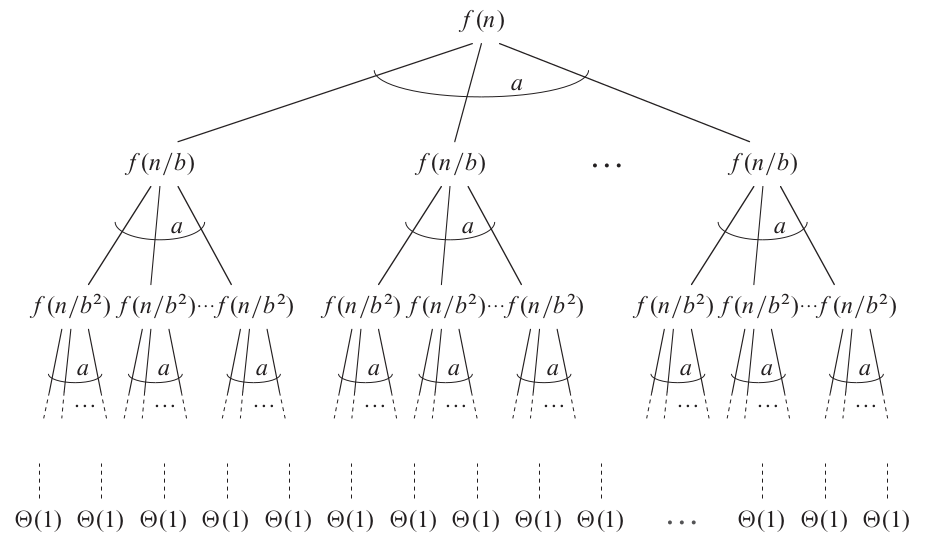
\includegraphics[width=\textwidth]{tree0}
\end{figure}
\end{center}
Question: What is the height of the tree?
\end{frame}

% Talking Points:
% - Show that the height is now there
% - The answer is a^{log_b n} because every node splits into a parts
%   - this happens |height| often
%   - Logarithmrules: this is the same as n^{log_b a}
\begin{frame}{Now a bit harder}
\begin{center}
\begin{figure}
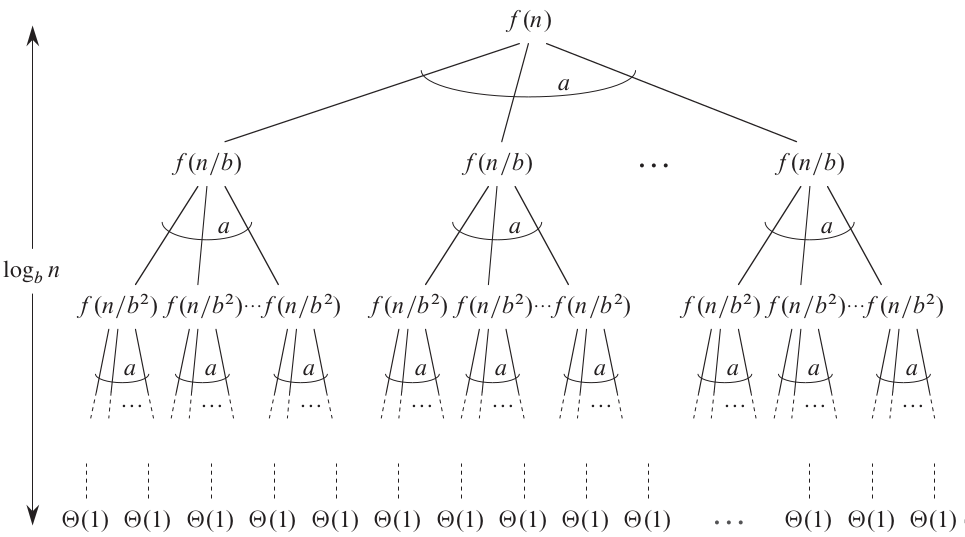
\includegraphics[width=\textwidth]{tree1}
\end{figure}
\end{center}
Question: Any idea how many leafes the tree could have?
\end{frame}

% Talking Points:
% - Depth 1: we have f(n/b), a times
% - Depth 2: For each subtree, we have f(n/b^2), a times.
% - and so on and so fourth
% - At the end, each node is Theta(1)
%   - We know the number of nodes, thus Theta(n^{log_b(a)})
%
% - After: The good thing about Big-O is that we can hide all smaller terms.
%    - Let's do that.
\begin{frame}{Let's sum it up depthwise.}
\begin{center}
\begin{figure}
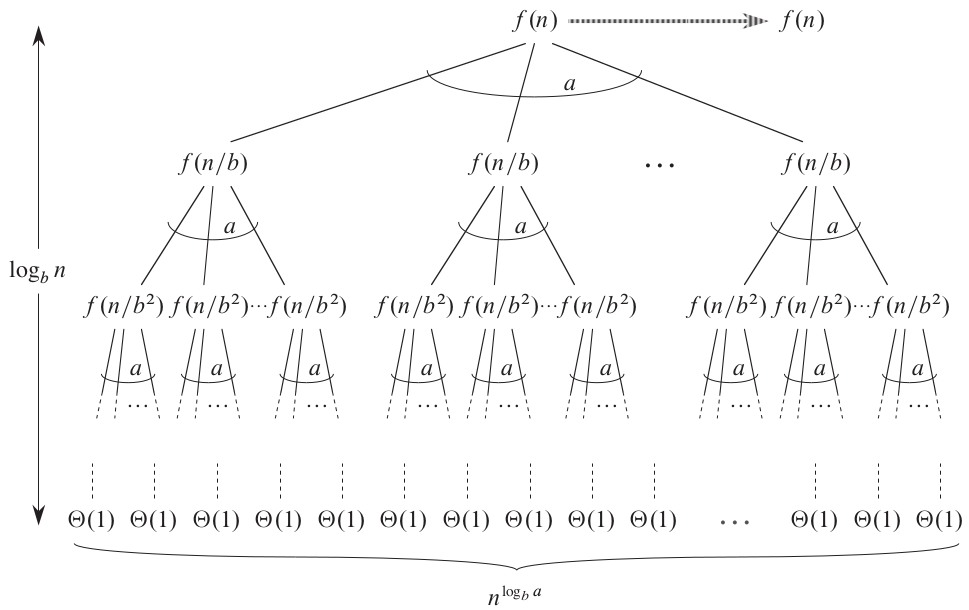
\includegraphics[width=\textwidth]{tree2}
\end{figure}
\end{center}
Question: Depth 0 has cost $f(n)$. What about the other depths?
\end{frame}

% Talking points:
% - After first pause:
%   - Obviously, we are working with Big(O), so it has to be at least polynomially smaller...
% - For second case:
%   - This means, that we need |hight| times the work
\begin{frame}{I think we can divide it into 3 cases.}
So, the total cost is
\[
T(n) = \Theta(n^{\log_b(a)}) + \sum_{j=0}^{\log_b(n) - 1} a^j f(n/b^j)
\]
\pause
This can be divided into 3 cases:
\begin{enumerate}
\item The cost is dominated by the cost in the leafes, i.e. $O(n^{\log_b(a)}) > \sum_{j=0}^{\log_b(n)-1}a^j f(n/b^j)$
\pause
\item The cost is evenly distributed, i.e. $O(n^{\log_b(a)}) \ni \sum_{j=0}^{\log_b(n)-1}a^j f(n/b^j)$
\pause
	\item The cost is dominated by the cost in the root i.e. $O(n^{\log_b(a)}) < \sum_{j=0}^{\log_b(n)-1}a^j f(n/b^j)$
\end{enumerate}
\end{frame}

% Talking points...
\begin{frame}{}
\begin{center}
I have seen that before...
\end{center}
\end{frame}

% Talking points:
% - If b not >1 then we have infinite runtime as the problem does not get smaller
% - 1. Case: it is dominated by the leafes
%    - The -\epsilon means that it is polynomially smaller, i.e. it can be hidden within
%
% - 2. Case: It is evenly distributed, thus the logarithm times the problem.
%
% - 3. Case: The extra condition is to be sure that the parent actually works as much as the children
%   - Otherwise, we couldn't hide the childrens complexity into the parent
%
% - We don't have enough time for the proof, even just for case 1.
%   - It's pretty easily described in Introduction to Algorithms, Chapter 4.4
%
% - Now let's use our new knowledge!
\begin{frame}{}
\begin{block}{Theorem 1: The Master Theorem}
Let $a \geq 1$ and $b > 1$ be constants, let $f(n)$ be a function, and let $T(n): \mathbb{N}_0 \rightarrow \mathbb{N}_0$
\[
T(n) = aT(n/b) + f(n)
\]
for powers of $2$. Then
\begin{enumerate}
\item If $f(n) = O(n^{\log_b(a) - \epsilon})$ for some constant $\epsilon > 0$, then $T(n) = \Theta(n^{\log_b(a)})$
\\~
\item If $f(n) = \Theta(n^{\log_b(a)})$, then $T(n) = \Theta(n^{\log_b(a)}\log(n))$
\\~
\item If $f(n) = \Omega(n^{\log_b(a)+\epsilon})$ for some constant $\epsilon > 0$ and if $af(n/b) \leq cf(n)$ for
some constant $c < 1$ and all sufficiently large $n$, then $T(n) = \Theta(f(n))$
\end{enumerate}
\end{block}
\end{frame}

% Talking point
\begin{frame}{}
\begin{block}{Theorem 2: Runtime Karatsuba's Multiplication}
The runtime of Karatsuba's Algorithm is $\Theta(n^{\log_2(3)}) \approx \Theta(n^{1.5849})$
\end{block}
\pause
\begin{proof}
\begin{itemize}
\item We did 3 Multiplication with a problem of size $n/2$ and did linear work adding it up
\[
T(n) = 3T(n/2) + \Theta(n)
\]
\pause
\item We know that $\Theta(n) \in O(n^{\log_2(3) - \epsilon})$ for some $\epsilon > 0$
\pause
\item Proven via master theorem, case 1.
\end{itemize}
\end{proof}
\end{frame}{}

\section{Generalization}

% Talking points:
\begin{frame}{The Toom-Cook Algorithm}
\begin{itemize}
\item The Toom-Cook Algorithm needs is kind of a weird algorithm
\pause
\begin{itemize}
\item It has a way bigger constant time
\pause
\item Sch\"onhage-Stra\ss{}en is near linear with not that much more overhead
\pause
\item It requires way more rigour to formalize;\\
it needs to be formalized on a case-by-case basis
\end{itemize}
\item I'll just sketch it out and show it's time complexity
\end{itemize}
\end{frame}

% Talking points:
% - Toom-2 is equivalent to Karatsuba but with bigger overhead.
\begin{frame}{The general idea}
\begin{itemize}
\item We can split up into more than $2$ parts!
\pause
\item The most used case is Toom-3, i.e. splitting up into 3 parts.\\
The recursion would look like
\[
T(n) = aT(n/3) + \Theta(n)
\]
\pause
\item If we get $a<9$, we get $\Theta(n^{\log_3(a)}) < \Theta(n^2)$, thus beating normal multiplication.
\pause
\item Let's see how they try to beat it.
\end{itemize}
\end{frame}

% Talking points:
% - Splitting:
%   - p' is equal to p, we just use factor out the unknown
% - Choosing:
%   - We know from numerical analysis that any polynomial of degree n
%     has n+1 degrees of freedom, thus we need n+1 points to define it.
%   - When done correctly, we can isolate the single terms
% - Evaluate: This is our recursion
% - Interpolate:
%   - From this 5 evaluations we get a linear system of equations
%   - If points were chosen well, this becomes a vandermonde matrix
%   - We can precompute it's inverse, then it is just a matrix-vector multiplication
\begin{frame}{The steps}

Toom-3 is divided in 5 steps:
\pause
\begin{enumerate}
\item Splitting the polynomials into $3$ even parts, i.e.
\[
p = p' := p'_2 x^2 + p'_1 x + p'_0
\]
\pause
\item Choose $\deg{pq}+1 = \deg{p}+\deg{q}+1$ points to interpolate it later
\pause
\item Evaluate these $5$ big multiplications for $pq$ recursively
\pause
\item Interpolate with the 5 evaluated points
\pause
\item Add up the result
\end{enumerate}
\pause
When done in a smart way, we just need 5 multipliations.
\end{frame}

% Talking points
\begin{frame}{}
\begin{block}{Theorem 3: Time Complexity Toom-3}
The time complexity of Toom-3 is $\Theta(n^{\log_3(5)}) \approx \Theta(n^{1.46})$
\end{block}
\pause
\begin{proof}
We need 5 multiplications and divide the problem into 3 even parts.\\
All other work in linear.\\
Thus
\[
T(n) = 5T(n/5) + \Theta(n)
\]
It follows from the master theorem, case 1.
\end{proof}
\end{frame}

\section{Beyond}

% Talking points
% - The convolution theorem states that under suitable condition that the
%   fourier transform of a convolution is equal to the pointwise-product (f(x) * g(x))
%   of their fourier transforms
% - F\"urer: Note that K is not specified
% - Iterated Log: How many applications until it is under 1. This is basically constant at (5-7)
\begin{frame}{What happened after Toom-Cook}
\pause
\begin{itemize}
\item 1965: The FFT became popular
\pause
\item 1971: Sch\"onhage Stra\ss{}en:
\begin{itemize}
\item $O(N \log(N) \log(\log(N)))$
\end{itemize}
\pause
\item 2007: Martin F\"urer:
\begin{itemize}
\item $O(N \cdot \log(N) \cdot K^{\log^*(N)})$
\end{itemize}
\pause
\item 2019: Harvey \& van der Hoeven:
\begin{itemize}
\item $O(N \log(N))$
\item To be worth it: $n$ has to have $2^{1729^{12}}$ digits long.
\end{itemize}
\end{itemize}
\end{frame}

\begin{frame}{Sources: Books}
Books
\begin{itemize}
\item \href{https://doi.org/10.1017/CBO9781139856065}{Modern Computer Algebra}
\item \href{https://dl.acm.org/doi/book/10.5555/1614191}{Introduction to Algorithms}
\item \href{https://dl.acm.org/doi/book/10.5555/270146}{The Art of Computer Programming: Volume 2}
\end{itemize}
Videos
\begin{itemize}
\item MIT OCW: \href{https://www.youtube.com/watch?v=eCaXlAaN2uE&t=2538s}{Karatsuba}, \href{https://www.youtube.com/watch?v=whjt\_N9uYFI&t=2784s}{Master Method}
\item \href{https://www.youtube.com/watch?v=cCKOl5li6YM}{Neman: How Karatsuba's algorithm gave us new ways to multiply}
\end{itemize}
Other:
\begin{itemize}
\item \href{https://gmplib.org/manual/Toom-3\_002dWay-Multiplication}{The GMP manual: 15.1.3 Toom 3-Way Multiplication}
\end{itemize}
\end{frame}


















{
  \usebackgroundtemplate{
  
\includegraphics[height=\paperheight,width=\paperwidth]{theend.jpg}
  }
  \begin{frame}[plain]
  \end{frame}
}
\end{document}
